%%%%%%%%%%%%%%%%%%%%%%%%%%%%%%%%%%%%%%%%%%%%%%%%%%
%% Authors :    Giovanni Arcari                 %%
%%              Mariia Bronzova                  %%
%%              Luca Sardi                      %%
%%              Spencer Sharp                   %%
%%                                              %%
%% Supervisor : Andreas Apostolatos             %%
%%											  	%%
%% e-mail : andreas.apostolatos@tum.de		   	%%
%%											  	%%
%% 02_Theoretical_background.tex				%%
%%											  	%%
%%%%%%%%%%%%%%%%%%%%%%%%%%%%%%%%%%%%%%%%%%%%%%%%%%
\section{THEORETICAL BACKGROUND}
\subsection{What is a Sensitivity Analysis?}
In general, a sensitivity analysis is a study on how output variables change according to a modification of the input parameter. In the field of structural analysis, it is used to determine the gradient of a response function which are used as objective or constraint. \\[3pt]
In the design process, this naturally leads to optimization: through a modification of the input data, an influence on the performance of the structure can be observed. \\[3pt]
In this report, a response sensitivity analysis will be taken into account.\\

\subsection{Response sensitivity analysis}
In general, optimal designs are characterized by the \textit{Karush-Kuhn-Tucker} condition, which, from \cite{optimization_Bletzinger}, states
\begin{equation}
\dv{L}{\textbf{x}} = \dv{f}{\textbf{x}} + \lambda^T  \dv{\textbf{g}}{\textbf{x}} 
%Lambda should be Bold
\end{equation}
where $f$ represents the objective function, $\textbf{g}$ the constraints and $\textbf{x}$ the optimization variables.
In general, structural response functions $f$ and $g$ depend on the design variables $\textbf{x}$ as well as the response variables $\textbf{u}$ which are usually represented by the structural displacements. \\
In mathematical terms, this is represented by the following relationships: 
\begin{equation}
f = f \big(\textbf{u}, \textbf{u(x)}\big)
\end{equation}
According to the chain rule, the differentiation of the objective function with respect to the design variables is
\begin{equation}
\dv{f}{\textbf{x}} = \pdv{f}{\textbf{x}} + \pdv{f}{\textbf{u}} \dv{\textbf{u}}{\textbf{x}}
\end{equation}

\subsection{Sensitivity of the response variables}
As said, in response sensitivity analysis the response variables \textbf{u} are represented by the nodal displacements, and the main task is to find the derivative of \textbf{u} with respect to the design variables \textbf{x}.\\[3pt]
Considering a typical displacement formulation of the finite elements method, the equilibrium condition is represented by 
\begin{equation}
\textbf{K}\textbf{u} = \textbf{P}
\end{equation}
where 
\begin{itemize}
\item \textbf{K}: system stiffness matrix 
\item \textbf{u}: vector of nodal displacements
\item \textbf{P}: load vector
\end{itemize}
From \cite{optimization_Bletzinger}, derivation with respect to \textbf{x} yields 
\begin{equation}
\dv{(\textbf{K}\textbf{u})}{\textbf{x}} = \dv{\textbf{P}}{\textbf{x}}
\end{equation}
\begin{equation}
\dv{\textbf{K}}{x}\textbf{u} + \textbf{K} \dv{\textbf{u}}{\textbf{x}} = \dv{\textbf{P}}{\textbf{x}}
\end{equation}
\begin{equation} \label{eqn:dudxSensitivity}
\dv{\textbf{u}}{\textbf{x}} = \textbf{K}^{-1} \Big(\dv{\textbf{P}}{\textbf{x}} - \dv{\textbf{K}}{\textbf{x}} \textbf{u}\Big)
\end{equation}
where $\Big(\dv{\textbf{P}}{\textbf{x}} - \dv{\textbf{K}}{\textbf{x}} \textbf{u}\Big)$ from Equation \ref{eqn:dudxSensitivity} is called the \textit{pseudo force vector} $\textbf{P}^{\ast}$.

\subsection{Analytical sensitivity analysis - direct method}
First of all, a direct approach is taken into account. This means that, in order to approximate the derivative of a response function, $g_j(\textbf{x}, \textbf{u}(\textbf{x}))$ with respect to $x_i$, i.e. (from \cite{optimization_Bletzinger}):
\begin{equation} \label{eqn:responsefctderivative}
\dv{g_j}{x_i} = \pdv{g_j}{x_i} + \pdv{g_j}{\textbf{u}} \pdv{\textbf{u}}{x_i} = \pdv{g_j}{x_i} + \pdv{g_j}{\textbf{u}} \textbf{K}^{-1} \Big(\dv{\textbf{P}}{x_i} - \dv{\textbf{K}}{x_i}\textbf{u}\Big)
\end{equation}
which means that, through a direct approach, 
\begin {itemize}
\item first, $\dv{\textbf{u}}{x_i}$ is computed by solving $\textbf{K}^{-1}\textbf{P}_i^{\ast}$;
\item then, $\dv{\textbf{u}}{x_i}$ is substituted into equation \ref{eqn:responsefctderivative}. $\textbf{K}^{-1}\textbf{P}_i^{\ast}$ needs to be solved $n$ times, where $n$ represents the number of design variables.
\end{itemize}

\subsection{Analytical sensitivity analysis - adjoint method}
Otherwise, the operation order can be reversed. The starting point, as illustrated before, is still the following: 
\begin{equation}
\dv{g_j}{x_i} = \pdv{g_j}{x_i} + \Big[\pdv{g_j}{\textbf{u}}\textbf{K}^{-1}\Big] \Big(\dv{\textbf{P}}{x_i} - \dv{\textbf{K}}{x_i}\textbf{u}\Big)
\end{equation}
From \cite{optimization_Bletzinger}, the \textit{adjoint variables} $\widetilde{\textbf{u}}_j$ can be calculated as 
\begin{equation} \label{eqn:adjointVariable}
\widetilde{\textbf{u}}_j = \textbf{K}^{-1} \pdv{g_j}{\textbf{u}}
\end{equation}
and the results can be inserted into the remaining formula. \\[3pt]
Equation \ref{eqn:adjointVariable} above has to be solved $m$ times, where $m$ represents the number of response functions $g_j$.

\subsection{Direct vs. adjoint method}
The optimal approach for a given problem will depend on its relative number of design variables, $n$ and response functions, $m$. If $n<m$ (i.e., high number of response functions), then the direct method should be chosen. Conversely, if $n>m$ (i.e., high number of design variables), then the adjoint method should be chosen.\\[3pt]
For example, shape optimization problems with FE-based parametrization are almost always characterized by a large number of design variables and a small number of response functions.\cite{firl_dissertation} In such a case, the adjoint approach makes more sense from a computational perspective.\\[3pt]
It is worth noting that in both methods, a very significant benefit is that the stiffness matrix, $\textbf{K}$, must only be inverted once. It can then be stored in memory, and future iteration steps only require matrix multiplication, rather than matrix inversion.

\subsection{Finite difference approximation}
The complexity of the element formulation makes the sensitivity analysis very difficult, sometimes impossible, to code. For this reason, a finite element approximation is often used. \\[3pt]
The first order derivative of a function $f$ with respect to $x_i$ can be approximated by the formula 
\begin{equation} \label{eqn:finitedifference}
\pdv{f}{x_i} \cong \frac{f(x_i + \Delta x_i) - f(x_i)}{\Delta x_i}
\end{equation}
The following sections discuss two potential applications for this formula: the global approach and the semi-analytical approach.
\subsection{Global sensitivity analysis}
Equation \ref{eqn:finitedifference} can be used to directly calculate the sensitivity of a system without any analytical equations. Thus, implementation is very easy. However, the system must be completely solved once for each design variable. In contrast to the analytical approaches, the global analysis requires that the stiffness matrix, $\textbf{K}$, be inverted with each iteration step. Matrix inversion is significantly more expensive than matrix multiplication, thus making this approach very expensive as the number of design variables increases.

\subsection{Semi-analytical sensitivity analysis}
Since a global sensitivity analysis of a system is extremely expensive and a complete analytical assessment is difficult and/or impossible, semi-analytical approaches are often utilized. This means that a mixture of both analytical and numerical methods is considered: equations are developed analytically, then all derivatives are replaced by their numerical approximation.\cite{optimization_Bletzinger} This approach leverages the benefit of the analytical method (i.e., matrix multiplication instead of inversion) without its drawback (i.e., difficult implementation of complex differentiation). Therefore, no additional element code is needed. This combination of analytical equations with finite difference approximations of their derivatives is henceforth referred to as the \textit{numerical adjoint method}. \\[3pt]
Such a seemingly perfect solution comes at a cost, however. With traditional finite element analysis, error typically diminishes as the mesh is refined. In the case of the semi-analytical sensitivity analysis, error can actually increase as the mesh is refined. This error stems from the rigid body rotation behavior of the approximated stiffness matrix derivative, which is exaggerated as element size decreases.\cite{optimization_Bletzinger}

\subsection{Differencing schemes}
In the script, several differencing schemes are taken into account. 
In this section, a quick look at the possible different ones is taken. Three methods exist to approximate the derivative of a function, \textit{forward}, \textit{backward} and \textit{central} differencing.\\[3pt]
Considering the formula 
\begin{equation}
\pdv{f}{x_i} \cong \frac{f(x_i + \Delta x_i) - f(x_i)}{\Delta x_i}
\end{equation}
\begin{figure}[ht]
  \centering
  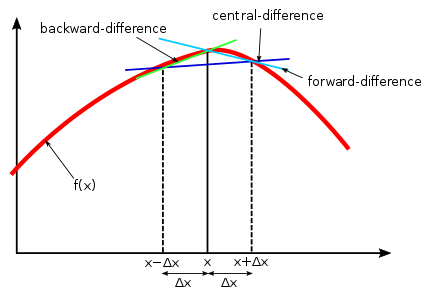
\includegraphics[width=110mm]{images/differencing.png}
  \caption{Visual illustration of differencing schemes\\ \cite{wiki:finiteDifference}}
  \label{fig:differencingschemes}
\end{figure}
In Figure \ref{fig:differencingschemes}, a visual representation of the differences between the approximation schemes is shown on a generic function taken as an example.
It is possible to see how the result of the approximation depends on the choice of $\Delta x_i$.
In particular, a step in the positive or negative direction can be taken, as well as in both of those. Respectively, these choices lead to forward, backward and central differencing method. \cite{masching_dissertation} \\[3pt]
Later on, it will be explained how the choice of the differencing scheme affects the results of the analysis.





